% Informe del laboratorio 3: control de versiones con Git/GitHub y modelo relacional (cierre de la fase 1)
% Compilar desde esta carpeta: pdflatex informe_lab03.tex (dos veces)
\documentclass[a4paper,11pt]{article}
% Preámbulo común de los informes de laboratorio (II/2026). Se incluye desde desarrollo/fuentes/laboratorios/labNN_*/
%   % Preámbulo común de los informes de laboratorio (II/2026). Se incluye desde desarrollo/fuentes/laboratorios/labNN_*/
%   % Preámbulo común de los informes de laboratorio (II/2026). Se incluye desde desarrollo/fuentes/laboratorios/labNN_*/
%   \input{../informe_comun}
\input{../../gemelo-digital/manual/estilo_manual}
\input{../../gemelo-digital/manual/tecnico/macros}
% Las rutas son relativas a la carpeta de cada informe (desarrollo/fuentes/laboratorios/labNN/): las fuentes
% (estilo, imágenes del manual, figuras y levantamiento) están en desarrollo/fuentes; los entregables públicos
% (planos, base de datos) cuatro niveles más arriba, en semestres/2026_II/.
\graphicspath{{../../../../documentacion/planos_isa/pid/}{../../../../documentacion/planos_isa/electrico/}{../../../../documentacion/manuales_inversa/}
  {../../../../database/mockups/}{../../../../database/documentacion/}{../../../../database/modelo/}{../../../../database/interfaz/}
  {../../gemelo-digital/manual/img/}{../../modelo-3d/informe/figuras/}{../../modelo-3d/levantamiento/}{../../../../../../global/fotos-planta/}}
\usepackage{pdflscape}
\lstset{showstringspaces=false}
% plano A3 en una página apaisada: \plano[página]{archivo}{leyenda}
\newcommand{\plano}[3][1]{\begin{landscape}\begin{figure}[p]\centering\includegraphics[page=#1, width=\linewidth, height=0.86\textwidth, keepaspectratio]{#2}\caption{#3}\end{figure}\end{landscape}}
\setlength{\headheight}{14pt}
\newcommand{\nlab}{}
\newcommand{\tlab}{}
% tipo de documento en la portada y el encabezado (los documentos de logros los redefinen)
\newcommand{\tipodoc}{Informe del Laboratorio Integrado}
\newcommand{\tipocab}{Informe del laboratorio}
\lhead{\small Brazo XK-JS1-1 · \tipocab{} \nlab}
\rhead{\small UMSA · II/2026}

% \portada{número}{título}{inicio}{entrega}{semanas}
\newcommand{\portada}[5]{%
\renewcommand{\nlab}{#1}%
\begin{titlepage}
\centering
\vspace*{0.6cm}
{\large Universidad Mayor de San Andrés · Facultad de Ingeniería\par}
{\large Carrera de Ingeniería Electrónica\par}
\vspace{0.8cm}
{\color{naranja!80!black}\rule{\linewidth}{1.5pt}\par}
\vspace{0.3cm}
{\Large \tipodoc{} Nº #1\par}
\vspace{0.2cm}
{\huge\bfseries #2\par}
\vspace{0.3cm}
{\color{naranja!80!black}\rule{\linewidth}{1.5pt}\par}
\vspace{0.8cm}
{\large Planta: brazo robótico XK-JS1-1 de 4 grados de libertad\par}
\vspace{0.3cm}
{\large ETN-902 Sistemas de Control II · ETN-1034 Aplicación de Técnicas de Control · ETN-1000 Bases de Datos\par}
\vspace{1cm}
\begin{tabular}{rl}
\textbf{Docente:} & Ing. Jorge Antonio Nava Amador\\
\textbf{Auxiliares:} & Limber Ajnota · Fabián Plata · Franz Choque\\
\textbf{Inicio de trabajo:} & #3\\
\textbf{Entrega:} & #4 (#5)\\
\end{tabular}
\vspace{1cm}

\begin{tabular}{ll}
\multicolumn{2}{l}{\textbf{Escuadra del brazo de 4 GDL}}\\[2pt]
Control (ETN-902 / ETN-1034): & Gabriel Andres Gomez Calla\\
 & Jose Lenin Mamani Choque\\
 & Miguel Alejandro Lima Huarachi\\
 & Román Abner Machicado Arequipa\\[2pt]
Cómputo (ETN-1000): & Miguel Alejandro Lima Huarachi\\
 & Marco Eduardo Chura Rondo\\
\end{tabular}
\vfill
{\small Repositorio: \url{https://github.com/GabAndGom/Brazo-de-4-grados-de-libertad}\par}
{\small La Paz, Bolivia · gestión II/2026\par}
\end{titlepage}
}

% Tabla de entregables (Definition of Done): \begin{dod} ... \end{dod}, filas: entregable & estado & evidencia\\
\newenvironment{dod}{\begin{center}\small\begin{longtable}{>{\raggedright}p{5.2cm} >{\raggedright}p{1.8cm} >{\raggedright\arraybackslash}p{7.6cm}}
\toprule \textbf{Entregable} & \textbf{Estado} & \textbf{Evidencia / observación}\\ \midrule \endhead}
{\bottomrule\end{longtable}\end{center}}

% Estilo común de los manuales del gemelo digital (se incluye con \input)
\usepackage{geometry}
\geometry{letterpaper, margin=2.2cm}
\usepackage[spanish, es-nodecimaldot, mexico]{babel}
\usepackage[utf8]{inputenc}
\usepackage[T1]{fontenc}
\usepackage{lmodern}
\usepackage{amsmath,amssymb}
\usepackage[table]{xcolor}
\definecolor{naranja}{RGB}{194,98,12}
\definecolor{rojo}{RGB}{192,57,43}
\definecolor{verde}{RGB}{30,120,70}
\definecolor{azulw}{RGB}{0,103,184}
\definecolor{azulg}{RGB}{70,90,120}
\definecolor{gris}{RGB}{242,242,242}
\definecolor{grisos}{RGB}{90,90,90}
\usepackage{booktabs,longtable,array,tabularx}
\usepackage{graphicx}
\usepackage{float}
\usepackage{caption}
\captionsetup{font=small, labelfont=bf}
\usepackage{tikz}
\usetikzlibrary{positioning,arrows.meta,fit,calc,shapes.geometric,decorations.pathreplacing,backgrounds}
\usepackage{enumitem}
\setlist{itemsep=2pt}
\usepackage{listings}
\lstset{basicstyle=\ttfamily\small, frame=single, backgroundcolor=\color{gris}, breaklines=true,
  columns=fullflexible, keepspaces=true, extendedchars=true, upquote=true,
  literate={á}{{\'a}}1 {é}{{\'e}}1 {í}{{\'i}}1 {ó}{{\'o}}1 {ú}{{\'u}}1 {ñ}{{\~n}}1 {Á}{{\'A}}1 {É}{{\'E}}1
           {Í}{{\'I}}1 {Ó}{{\'O}}1 {Ú}{{\'U}}1 {Ñ}{{\~N}}1 {ü}{{\"u}}1 {¿}{{?`}}1 {¡}{{!`}}1 {…}{{...}}3
           {θ}{{$\theta$}}1 {·}{{$\cdot$}}1 {«}{{\guillemotleft}}1 {»}{{\guillemotright}}1 {°}{{$^\circ$}}1}
\usepackage{hyperref}
\hypersetup{colorlinks=true, linkcolor=naranja, urlcolor=naranja}
\usepackage{fancyhdr}
\pagestyle{fancy}
\fancyhf{}
\cfoot{\small \thepage}
\newcommand{\codigo}[1]{\texttt{#1}}
\newcommand{\archivo}[1]{\textbf{\texttt{#1}}}
\newcommand{\aviso}[1]{\par\smallskip\noindent\colorbox{rojo!10}{\parbox{\dimexpr\linewidth-2\fboxsep}{\textbf{\color{rojo}Atención.} #1}}\par\smallskip}
\newcommand{\nota}[1]{\par\smallskip\noindent\colorbox{gris}{\parbox{\dimexpr\linewidth-2\fboxsep}{#1}}\par\smallskip}
\tikzset{
  marca/.style={circle, fill=naranja, text=white, font=\bfseries\footnotesize, inner sep=1.4pt, minimum size=4.6mm, draw=white, line width=0.8pt},
  caja/.style={draw, rounded corners=2pt, fill=gris, align=center, font=\small, minimum height=10mm, inner sep=4pt},
  cajab/.style={caja, fill=white},
  cajan/.style={caja, fill=naranja!14, draw=naranja!70!black},
  paso/.style={draw, rounded corners=2pt, fill=white, align=left, font=\small, text width=3.4cm, minimum height=15mm, inner sep=5pt},
  num/.style={circle, fill=naranja, text=white, font=\bfseries\small, inner sep=1.5pt, minimum size=6mm},
  flecha/.style={-{Stealth[length=2.2mm]}, thick},
  dflecha/.style={{Stealth[length=2.2mm]}-{Stealth[length=2.2mm]}, thick},
  etiq/.style={font=\scriptsize, align=center},
}
\DeclareRobustCommand{\num}[1]{\tikz[baseline=-0.7ex]\node[marca]{#1};}
% \captura{ancho}{archivo}{marcas en coordenadas 0-1 desde la esquina inferior izquierda}
\newcommand{\captura}[3]{%
  \begin{tikzpicture}
  \node[anchor=south west, inner sep=0, draw=black!25] (img) {\includegraphics[width=#1]{#2}};
  \begin{scope}[x={(img.south east)}, y={(img.north west)}]
  #3
  \end{scope}
  \end{tikzpicture}}
% ventana dibujada (consolas y diálogos): \ventana{ancho}{alto}{título}{contenido}
\newcommand{\ventana}[4]{%
\begin{tikzpicture}
\node[draw=black!50, fill=white, minimum width=#1, minimum height=#2, anchor=north west, inner sep=0] (v) at (0,0) {};
\fill[black!8] (v.north west) rectangle ($(v.north east)+(0,-6mm)$);
\node[anchor=west, font=\scriptsize] at ($(v.north west)+(2mm,-3mm)$) {#3};
\node[anchor=east, font=\scriptsize] at ($(v.north east)+(-2mm,-3mm)$) {--\quad$\square$\quad$\times$};
\node[anchor=north west, inner sep=3mm, text width=#1-6mm, font=\scriptsize\ttfamily, align=left] at ($(v.north west)+(0,-6mm)$) {#4};
\end{tikzpicture}}

% Macros del manual técnico: ladder, estados, código y rutas de imágenes
\usetikzlibrary{shapes.multipart}
\graphicspath{{../img/}{../../../../../../../global/fotos-planta/}{../../../modelo-3d/informe/figuras/}{../../../modelo-3d/levantamiento/}{../../../../../database/modelo/}{../../../../../documentacion/manuales_inversa/}{../../../../../documentacion/planos_isa/electrico/}{../../../../../database/interfaz/}}

\lstdefinestyle{py}{language=Python, keywordstyle=\color{azulg}\bfseries, commentstyle=\color{grisos}\itshape,
  stringstyle=\color{verde}, basicstyle=\ttfamily\scriptsize, numbers=left, numberstyle=\tiny\color{grisos}}
\lstdefinestyle{js}{language=Java, morekeywords={const,let,function,async,await,return,for,of,if,else}, keywordstyle=\color{azulg}\bfseries,
  commentstyle=\color{grisos}\itshape, stringstyle=\color{verde}, basicstyle=\ttfamily\scriptsize, numbers=left, numberstyle=\tiny\color{grisos}}
\lstdefinestyle{awl}{basicstyle=\ttfamily\tiny, commentstyle=\color{grisos}\itshape, morecomment=[l]{//},
  keywordstyle=\color{azulg}\bfseries, morekeywords={LD,LDN,A,AN,O,ON,EU,ED,S,R,MOVB,MOVW,MOVD,PLS,TON,CALL,CRET,LPS,LRD,LPP,ALD,OLD,FILL,LDW,LDB,LDD,AW,AD,AB,OW,OD},
  numbers=left, numberstyle=\tiny\color{grisos}, frame=single, backgroundcolor=\color{gris}}
\lstdefinestyle{sql}{language=SQL, keywordstyle=\color{azulg}\bfseries, commentstyle=\color{grisos}\itshape,
  stringstyle=\color{verde}, basicstyle=\ttfamily\tiny, numbers=left, numberstyle=\tiny\color{grisos},
  morekeywords={REFERENCES,SERIAL,SMALLSERIAL,BIGSERIAL,TIMESTAMPTZ,BOOLEAN,INET,RETURNS,TRIGGER,LANGUAGE,DECLARE,RAISE,EXCEPTION,VIEW,INDEX}}

\tikzset{
  ld/.style={line width=0.7pt},
  pics/na/.style={code={\fill[white](-0.12,-0.26) rectangle (0.12,0.26);
     \draw[thick](-0.1,-0.24)--(-0.1,0.24)(0.1,-0.24)--(0.1,0.24);
     \node[font=\scriptsize\ttfamily, above] at (0,0.22){#1};}},
  pics/nc/.style={code={\fill[white](-0.12,-0.26) rectangle (0.12,0.26);
     \draw[thick](-0.1,-0.24)--(-0.1,0.24)(0.1,-0.24)--(0.1,0.24);\draw(-0.17,-0.24)--(0.17,0.24);
     \node[font=\scriptsize\ttfamily, above] at (0,0.22){#1};}},
  pics/pf/.style={code={\fill[white](-0.12,-0.26) rectangle (0.12,0.26);
     \draw[thick](-0.1,-0.24)--(-0.1,0.24)(0.1,-0.24)--(0.1,0.24);
     \node[font=\tiny\bfseries] at (0,0){P};}},
  pics/cmp/.style n args={3}{code={\fill[white](-0.12,-0.26) rectangle (0.12,0.26);
     \draw[thick](-0.1,-0.24)--(-0.1,0.24)(0.1,-0.24)--(0.1,0.24);
     \node[font=\tiny\ttfamily] at (0,0){#2};
     \node[font=\scriptsize\ttfamily, above] at (0,0.22){#1};
     \node[font=\scriptsize\ttfamily, below] at (0,-0.22){#3};}},
  pics/bob/.style n args={3}{code={\fill[white](-0.2,-0.26) rectangle (0.2,0.26);
     \draw[thick](-0.05,0.24) arc (110:250:0.255);\draw[thick](0.05,0.24) arc (70:-70:0.255);
     \node[font=\tiny\bfseries] at (0,0){#2};
     \node[font=\scriptsize\ttfamily, above] at (0,0.22){#1};
     \node[font=\scriptsize\ttfamily, below] at (0,-0.22){#3};}},
  fb/.style={draw, fill=white, font=\scriptsize\ttfamily, align=left, inner sep=3pt, anchor=west},
  barra/.style={line width=2pt},
  estado/.style={draw, rounded corners=3pt, fill=white, align=center, font=\scriptsize, minimum width=22mm, minimum height=10mm, inner sep=3pt},
  estadon/.style={estado, fill=naranja!14, draw=naranja!70!black},
  trans/.style={font=\scriptsize, align=center, fill=white, inner sep=1pt},
  lugar/.style={circle, draw, thick, minimum size=7mm, fill=white},
  transicion/.style={rectangle, fill=black, minimum width=1.6mm, minimum height=7mm, inner sep=0},
  tabla/.style={rectangle split, rectangle split parts=2, draw, fill=white, font=\tiny\ttfamily, align=left, inner sep=2pt, rounded corners=1pt, text width=33mm},
}
\newcommand{\pendiente}[1]{\par\smallskip\noindent\colorbox{naranja!12}{\parbox{\dimexpr\linewidth-2\fboxsep}{\textbf{\color{naranja!80!black}Pendiente.} #1}}\par\smallskip}
\newcommand{\cumple}{\textcolor{verde}{\textbf{cumplido}}}
\newcommand{\parcial}{\textcolor{naranja}{\textbf{parcial}}}
\newcommand{\falta}{\textcolor{rojo}{\textbf{pendiente}}}

% Las rutas son relativas a la carpeta de cada informe (desarrollo/fuentes/laboratorios/labNN/): las fuentes
% (estilo, imágenes del manual, figuras y levantamiento) están en desarrollo/fuentes; los entregables públicos
% (planos, base de datos) cuatro niveles más arriba, en semestres/2026_II/.
\graphicspath{{../../../../documentacion/planos_isa/pid/}{../../../../documentacion/planos_isa/electrico/}{../../../../documentacion/manuales_inversa/}
  {../../../../database/mockups/}{../../../../database/documentacion/}{../../../../database/modelo/}{../../../../database/interfaz/}
  {../../gemelo-digital/manual/img/}{../../modelo-3d/informe/figuras/}{../../modelo-3d/levantamiento/}{../../../../../../global/fotos-planta/}}
\usepackage{pdflscape}
\lstset{showstringspaces=false}
% plano A3 en una página apaisada: \plano[página]{archivo}{leyenda}
\newcommand{\plano}[3][1]{\begin{landscape}\begin{figure}[p]\centering\includegraphics[page=#1, width=\linewidth, height=0.86\textwidth, keepaspectratio]{#2}\caption{#3}\end{figure}\end{landscape}}
\setlength{\headheight}{14pt}
\newcommand{\nlab}{}
\newcommand{\tlab}{}
% tipo de documento en la portada y el encabezado (los documentos de logros los redefinen)
\newcommand{\tipodoc}{Informe del Laboratorio Integrado}
\newcommand{\tipocab}{Informe del laboratorio}
\lhead{\small Brazo XK-JS1-1 · \tipocab{} \nlab}
\rhead{\small UMSA · II/2026}

% \portada{número}{título}{inicio}{entrega}{semanas}
\newcommand{\portada}[5]{%
\renewcommand{\nlab}{#1}%
\begin{titlepage}
\centering
\vspace*{0.6cm}
{\large Universidad Mayor de San Andrés · Facultad de Ingeniería\par}
{\large Carrera de Ingeniería Electrónica\par}
\vspace{0.8cm}
{\color{naranja!80!black}\rule{\linewidth}{1.5pt}\par}
\vspace{0.3cm}
{\Large \tipodoc{} Nº #1\par}
\vspace{0.2cm}
{\huge\bfseries #2\par}
\vspace{0.3cm}
{\color{naranja!80!black}\rule{\linewidth}{1.5pt}\par}
\vspace{0.8cm}
{\large Planta: brazo robótico XK-JS1-1 de 4 grados de libertad\par}
\vspace{0.3cm}
{\large ETN-902 Sistemas de Control II · ETN-1034 Aplicación de Técnicas de Control · ETN-1000 Bases de Datos\par}
\vspace{1cm}
\begin{tabular}{rl}
\textbf{Docente:} & Ing. Jorge Antonio Nava Amador\\
\textbf{Auxiliares:} & Limber Ajnota · Fabián Plata · Franz Choque\\
\textbf{Inicio de trabajo:} & #3\\
\textbf{Entrega:} & #4 (#5)\\
\end{tabular}
\vspace{1cm}

\begin{tabular}{ll}
\multicolumn{2}{l}{\textbf{Escuadra del brazo de 4 GDL}}\\[2pt]
Control (ETN-902 / ETN-1034): & Gabriel Andres Gomez Calla\\
 & Jose Lenin Mamani Choque\\
 & Miguel Alejandro Lima Huarachi\\
 & Román Abner Machicado Arequipa\\[2pt]
Cómputo (ETN-1000): & Miguel Alejandro Lima Huarachi\\
 & Marco Eduardo Chura Rondo\\
\end{tabular}
\vfill
{\small Repositorio: \url{https://github.com/GabAndGom/Brazo-de-4-grados-de-libertad}\par}
{\small La Paz, Bolivia · gestión II/2026\par}
\end{titlepage}
}

% Tabla de entregables (Definition of Done): \begin{dod} ... \end{dod}, filas: entregable & estado & evidencia\\
\newenvironment{dod}{\begin{center}\small\begin{longtable}{>{\raggedright}p{5.2cm} >{\raggedright}p{1.8cm} >{\raggedright\arraybackslash}p{7.6cm}}
\toprule \textbf{Entregable} & \textbf{Estado} & \textbf{Evidencia / observación}\\ \midrule \endhead}
{\bottomrule\end{longtable}\end{center}}

% Estilo común de los manuales del gemelo digital (se incluye con \input)
\usepackage{geometry}
\geometry{letterpaper, margin=2.2cm}
\usepackage[spanish, es-nodecimaldot, mexico]{babel}
\usepackage[utf8]{inputenc}
\usepackage[T1]{fontenc}
\usepackage{lmodern}
\usepackage{amsmath,amssymb}
\usepackage[table]{xcolor}
\definecolor{naranja}{RGB}{194,98,12}
\definecolor{rojo}{RGB}{192,57,43}
\definecolor{verde}{RGB}{30,120,70}
\definecolor{azulw}{RGB}{0,103,184}
\definecolor{azulg}{RGB}{70,90,120}
\definecolor{gris}{RGB}{242,242,242}
\definecolor{grisos}{RGB}{90,90,90}
\usepackage{booktabs,longtable,array,tabularx}
\usepackage{graphicx}
\usepackage{float}
\usepackage{caption}
\captionsetup{font=small, labelfont=bf}
\usepackage{tikz}
\usetikzlibrary{positioning,arrows.meta,fit,calc,shapes.geometric,decorations.pathreplacing,backgrounds}
\usepackage{enumitem}
\setlist{itemsep=2pt}
\usepackage{listings}
\lstset{basicstyle=\ttfamily\small, frame=single, backgroundcolor=\color{gris}, breaklines=true,
  columns=fullflexible, keepspaces=true, extendedchars=true, upquote=true,
  literate={á}{{\'a}}1 {é}{{\'e}}1 {í}{{\'i}}1 {ó}{{\'o}}1 {ú}{{\'u}}1 {ñ}{{\~n}}1 {Á}{{\'A}}1 {É}{{\'E}}1
           {Í}{{\'I}}1 {Ó}{{\'O}}1 {Ú}{{\'U}}1 {Ñ}{{\~N}}1 {ü}{{\"u}}1 {¿}{{?`}}1 {¡}{{!`}}1 {…}{{...}}3
           {θ}{{$\theta$}}1 {·}{{$\cdot$}}1 {«}{{\guillemotleft}}1 {»}{{\guillemotright}}1 {°}{{$^\circ$}}1}
\usepackage{hyperref}
\hypersetup{colorlinks=true, linkcolor=naranja, urlcolor=naranja}
\usepackage{fancyhdr}
\pagestyle{fancy}
\fancyhf{}
\cfoot{\small \thepage}
\newcommand{\codigo}[1]{\texttt{#1}}
\newcommand{\archivo}[1]{\textbf{\texttt{#1}}}
\newcommand{\aviso}[1]{\par\smallskip\noindent\colorbox{rojo!10}{\parbox{\dimexpr\linewidth-2\fboxsep}{\textbf{\color{rojo}Atención.} #1}}\par\smallskip}
\newcommand{\nota}[1]{\par\smallskip\noindent\colorbox{gris}{\parbox{\dimexpr\linewidth-2\fboxsep}{#1}}\par\smallskip}
\tikzset{
  marca/.style={circle, fill=naranja, text=white, font=\bfseries\footnotesize, inner sep=1.4pt, minimum size=4.6mm, draw=white, line width=0.8pt},
  caja/.style={draw, rounded corners=2pt, fill=gris, align=center, font=\small, minimum height=10mm, inner sep=4pt},
  cajab/.style={caja, fill=white},
  cajan/.style={caja, fill=naranja!14, draw=naranja!70!black},
  paso/.style={draw, rounded corners=2pt, fill=white, align=left, font=\small, text width=3.4cm, minimum height=15mm, inner sep=5pt},
  num/.style={circle, fill=naranja, text=white, font=\bfseries\small, inner sep=1.5pt, minimum size=6mm},
  flecha/.style={-{Stealth[length=2.2mm]}, thick},
  dflecha/.style={{Stealth[length=2.2mm]}-{Stealth[length=2.2mm]}, thick},
  etiq/.style={font=\scriptsize, align=center},
}
\DeclareRobustCommand{\num}[1]{\tikz[baseline=-0.7ex]\node[marca]{#1};}
% \captura{ancho}{archivo}{marcas en coordenadas 0-1 desde la esquina inferior izquierda}
\newcommand{\captura}[3]{%
  \begin{tikzpicture}
  \node[anchor=south west, inner sep=0, draw=black!25] (img) {\includegraphics[width=#1]{#2}};
  \begin{scope}[x={(img.south east)}, y={(img.north west)}]
  #3
  \end{scope}
  \end{tikzpicture}}
% ventana dibujada (consolas y diálogos): \ventana{ancho}{alto}{título}{contenido}
\newcommand{\ventana}[4]{%
\begin{tikzpicture}
\node[draw=black!50, fill=white, minimum width=#1, minimum height=#2, anchor=north west, inner sep=0] (v) at (0,0) {};
\fill[black!8] (v.north west) rectangle ($(v.north east)+(0,-6mm)$);
\node[anchor=west, font=\scriptsize] at ($(v.north west)+(2mm,-3mm)$) {#3};
\node[anchor=east, font=\scriptsize] at ($(v.north east)+(-2mm,-3mm)$) {--\quad$\square$\quad$\times$};
\node[anchor=north west, inner sep=3mm, text width=#1-6mm, font=\scriptsize\ttfamily, align=left] at ($(v.north west)+(0,-6mm)$) {#4};
\end{tikzpicture}}

% Macros del manual técnico: ladder, estados, código y rutas de imágenes
\usetikzlibrary{shapes.multipart}
\graphicspath{{../img/}{../../../../../../../global/fotos-planta/}{../../../modelo-3d/informe/figuras/}{../../../modelo-3d/levantamiento/}{../../../../../database/modelo/}{../../../../../documentacion/manuales_inversa/}{../../../../../documentacion/planos_isa/electrico/}{../../../../../database/interfaz/}}

\lstdefinestyle{py}{language=Python, keywordstyle=\color{azulg}\bfseries, commentstyle=\color{grisos}\itshape,
  stringstyle=\color{verde}, basicstyle=\ttfamily\scriptsize, numbers=left, numberstyle=\tiny\color{grisos}}
\lstdefinestyle{js}{language=Java, morekeywords={const,let,function,async,await,return,for,of,if,else}, keywordstyle=\color{azulg}\bfseries,
  commentstyle=\color{grisos}\itshape, stringstyle=\color{verde}, basicstyle=\ttfamily\scriptsize, numbers=left, numberstyle=\tiny\color{grisos}}
\lstdefinestyle{awl}{basicstyle=\ttfamily\tiny, commentstyle=\color{grisos}\itshape, morecomment=[l]{//},
  keywordstyle=\color{azulg}\bfseries, morekeywords={LD,LDN,A,AN,O,ON,EU,ED,S,R,MOVB,MOVW,MOVD,PLS,TON,CALL,CRET,LPS,LRD,LPP,ALD,OLD,FILL,LDW,LDB,LDD,AW,AD,AB,OW,OD},
  numbers=left, numberstyle=\tiny\color{grisos}, frame=single, backgroundcolor=\color{gris}}
\lstdefinestyle{sql}{language=SQL, keywordstyle=\color{azulg}\bfseries, commentstyle=\color{grisos}\itshape,
  stringstyle=\color{verde}, basicstyle=\ttfamily\tiny, numbers=left, numberstyle=\tiny\color{grisos},
  morekeywords={REFERENCES,SERIAL,SMALLSERIAL,BIGSERIAL,TIMESTAMPTZ,BOOLEAN,INET,RETURNS,TRIGGER,LANGUAGE,DECLARE,RAISE,EXCEPTION,VIEW,INDEX}}

\tikzset{
  ld/.style={line width=0.7pt},
  pics/na/.style={code={\fill[white](-0.12,-0.26) rectangle (0.12,0.26);
     \draw[thick](-0.1,-0.24)--(-0.1,0.24)(0.1,-0.24)--(0.1,0.24);
     \node[font=\scriptsize\ttfamily, above] at (0,0.22){#1};}},
  pics/nc/.style={code={\fill[white](-0.12,-0.26) rectangle (0.12,0.26);
     \draw[thick](-0.1,-0.24)--(-0.1,0.24)(0.1,-0.24)--(0.1,0.24);\draw(-0.17,-0.24)--(0.17,0.24);
     \node[font=\scriptsize\ttfamily, above] at (0,0.22){#1};}},
  pics/pf/.style={code={\fill[white](-0.12,-0.26) rectangle (0.12,0.26);
     \draw[thick](-0.1,-0.24)--(-0.1,0.24)(0.1,-0.24)--(0.1,0.24);
     \node[font=\tiny\bfseries] at (0,0){P};}},
  pics/cmp/.style n args={3}{code={\fill[white](-0.12,-0.26) rectangle (0.12,0.26);
     \draw[thick](-0.1,-0.24)--(-0.1,0.24)(0.1,-0.24)--(0.1,0.24);
     \node[font=\tiny\ttfamily] at (0,0){#2};
     \node[font=\scriptsize\ttfamily, above] at (0,0.22){#1};
     \node[font=\scriptsize\ttfamily, below] at (0,-0.22){#3};}},
  pics/bob/.style n args={3}{code={\fill[white](-0.2,-0.26) rectangle (0.2,0.26);
     \draw[thick](-0.05,0.24) arc (110:250:0.255);\draw[thick](0.05,0.24) arc (70:-70:0.255);
     \node[font=\tiny\bfseries] at (0,0){#2};
     \node[font=\scriptsize\ttfamily, above] at (0,0.22){#1};
     \node[font=\scriptsize\ttfamily, below] at (0,-0.22){#3};}},
  fb/.style={draw, fill=white, font=\scriptsize\ttfamily, align=left, inner sep=3pt, anchor=west},
  barra/.style={line width=2pt},
  estado/.style={draw, rounded corners=3pt, fill=white, align=center, font=\scriptsize, minimum width=22mm, minimum height=10mm, inner sep=3pt},
  estadon/.style={estado, fill=naranja!14, draw=naranja!70!black},
  trans/.style={font=\scriptsize, align=center, fill=white, inner sep=1pt},
  lugar/.style={circle, draw, thick, minimum size=7mm, fill=white},
  transicion/.style={rectangle, fill=black, minimum width=1.6mm, minimum height=7mm, inner sep=0},
  tabla/.style={rectangle split, rectangle split parts=2, draw, fill=white, font=\tiny\ttfamily, align=left, inner sep=2pt, rounded corners=1pt, text width=33mm},
}
\newcommand{\pendiente}[1]{\par\smallskip\noindent\colorbox{naranja!12}{\parbox{\dimexpr\linewidth-2\fboxsep}{\textbf{\color{naranja!80!black}Pendiente.} #1}}\par\smallskip}
\newcommand{\cumple}{\textcolor{verde}{\textbf{cumplido}}}
\newcommand{\parcial}{\textcolor{naranja}{\textbf{parcial}}}
\newcommand{\falta}{\textcolor{rojo}{\textbf{pendiente}}}

% Las rutas son relativas a la carpeta de cada informe (desarrollo/fuentes/laboratorios/labNN/): las fuentes
% (estilo, imágenes del manual, figuras y levantamiento) están en desarrollo/fuentes; los entregables públicos
% (planos, base de datos) cuatro niveles más arriba, en semestres/2026_II/.
\graphicspath{{../../../../documentacion/planos_isa/pid/}{../../../../documentacion/planos_isa/electrico/}{../../../../documentacion/manuales_inversa/}
  {../../../../database/mockups/}{../../../../database/documentacion/}{../../../../database/modelo/}{../../../../database/interfaz/}
  {../../gemelo-digital/manual/img/}{../../modelo-3d/informe/figuras/}{../../modelo-3d/levantamiento/}{../../../../../../global/fotos-planta/}}
\usepackage{pdflscape}
\lstset{showstringspaces=false}
% plano A3 en una página apaisada: \plano[página]{archivo}{leyenda}
\newcommand{\plano}[3][1]{\begin{landscape}\begin{figure}[p]\centering\includegraphics[page=#1, width=\linewidth, height=0.86\textwidth, keepaspectratio]{#2}\caption{#3}\end{figure}\end{landscape}}
\setlength{\headheight}{14pt}
\newcommand{\nlab}{}
\newcommand{\tlab}{}
% tipo de documento en la portada y el encabezado (los documentos de logros los redefinen)
\newcommand{\tipodoc}{Informe del Laboratorio Integrado}
\newcommand{\tipocab}{Informe del laboratorio}
\lhead{\small Brazo XK-JS1-1 · \tipocab{} \nlab}
\rhead{\small UMSA · II/2026}

% \portada{número}{título}{inicio}{entrega}{semanas}
\newcommand{\portada}[5]{%
\renewcommand{\nlab}{#1}%
\begin{titlepage}
\centering
\vspace*{0.6cm}
{\large Universidad Mayor de San Andrés · Facultad de Ingeniería\par}
{\large Carrera de Ingeniería Electrónica\par}
\vspace{0.8cm}
{\color{naranja!80!black}\rule{\linewidth}{1.5pt}\par}
\vspace{0.3cm}
{\Large \tipodoc{} Nº #1\par}
\vspace{0.2cm}
{\huge\bfseries #2\par}
\vspace{0.3cm}
{\color{naranja!80!black}\rule{\linewidth}{1.5pt}\par}
\vspace{0.8cm}
{\large Planta: brazo robótico XK-JS1-1 de 4 grados de libertad\par}
\vspace{0.3cm}
{\large ETN-902 Sistemas de Control II · ETN-1034 Aplicación de Técnicas de Control · ETN-1000 Bases de Datos\par}
\vspace{1cm}
\begin{tabular}{rl}
\textbf{Docente:} & Ing. Jorge Antonio Nava Amador\\
\textbf{Auxiliares:} & Limber Ajnota · Fabián Plata · Franz Choque\\
\textbf{Inicio de trabajo:} & #3\\
\textbf{Entrega:} & #4 (#5)\\
\end{tabular}
\vspace{1cm}

\begin{tabular}{ll}
\multicolumn{2}{l}{\textbf{Escuadra del brazo de 4 GDL}}\\[2pt]
Control (ETN-902 / ETN-1034): & Gabriel Andres Gomez Calla\\
 & Jose Lenin Mamani Choque\\
 & Miguel Alejandro Lima Huarachi\\
 & Román Abner Machicado Arequipa\\[2pt]
Cómputo (ETN-1000): & Miguel Alejandro Lima Huarachi\\
 & Marco Eduardo Chura Rondo\\
\end{tabular}
\vfill
{\small Repositorio: \url{https://github.com/GabAndGom/Brazo-de-4-grados-de-libertad}\par}
{\small La Paz, Bolivia · gestión II/2026\par}
\end{titlepage}
}

% Tabla de entregables (Definition of Done): \begin{dod} ... \end{dod}, filas: entregable & estado & evidencia\\
\newenvironment{dod}{\begin{center}\small\begin{longtable}{>{\raggedright}p{5.2cm} >{\raggedright}p{1.8cm} >{\raggedright\arraybackslash}p{7.6cm}}
\toprule \textbf{Entregable} & \textbf{Estado} & \textbf{Evidencia / observación}\\ \midrule \endhead}
{\bottomrule\end{longtable}\end{center}}


\begin{document}
\portada{3}{Control de versiones y modelo relacional de datos · cierre de la fase 1}{martes 1 de septiembre de 2026}{martes 15 de septiembre de 2026}{semanas 5 y 6}

\tableofcontents
\newpage

\section{Introducción}
El laboratorio 3 cierra la fase 1. Lleva el trabajo de la escuadra al entorno informático con dos ejes: un flujo formal de control de versiones con Git y GitHub para custodiar la evolución de los planos, los programas y la documentación bajo la filosofía Kaizen; y la formalización del modelo entidad--relación preliminar del laboratorio 1 en un modelo normalizado (1FN, 2FN y 3FN) con su modelo lógico, implementado en PostgreSQL.

\begin{itemize}
\item \textbf{Laboratorio 1}: auditoría física y levantamiento de requerimientos; diagnóstico de lazo abierto con supervisión discreta y reporte de discrepancias Kaizen.
\item \textbf{Laboratorio 2}: P\&ID (ISA-5.1) y esquema eléctrico (IEC 60617) versión 2.0, mockups de la HMI y del dashboard.
\item \textbf{Laboratorio 3}: control de versiones, estructura del repositorio y modelo relacional en 3FN.
\end{itemize}

\section{Objetivos}
\subsection{Mención Control Automático (ETN-902 / ETN-1034)}
\begin{itemize}
\item \textbf{Gestión del ciclo de vida del software de control}: custodiar la documentación y los programas con Git y GitHub, con commits descriptivos, ramas y revisión técnica.
\item \textbf{Gestión de cambios de ingeniería (Kaizen)}: consolidar la versión 2.0 de los planos con un flujo formal de revisión y aprobación (Pull Requests) que evite pérdidas o duplicaciones entre gestiones.
\end{itemize}
\subsection{Mención Sistemas Computacionales (ETN-1000)}
\begin{itemize}
\item \textbf{Modelado relacional}: transformar los requerimientos de telemetría y los mockups en un modelo E-R formal y su modelo lógico, normalizados hasta 3FN.
\item \textbf{Estandarización del repositorio}: diseñar la estructura de carpetas para que base de datos, middleware y archivos CAD convivan de forma modular y documentada.
\end{itemize}

\section{Alcance}
El laboratorio se ejecutó en el laboratorio de cómputo, sin conexiones eléctricas ni neumáticas en caliente sobre la planta. Las computadoras se usaron para el control de versiones y la emulación local de la base de datos. Los integrantes trabajan en Windows, por eso el flujo se estandarizó sobre Git Bash.

\section{Marco teórico}
\subsection{Control de versiones con Git}
Un sistema de control de versiones registra los cambios de un conjunto de archivos a lo largo del tiempo: permite recuperar versiones, comparar diferencias y coordinar a varios colaboradores. Git es distribuido: cada colaborador tiene el historial completo. Sus conceptos básicos son:
\begin{itemize}
\item \textbf{repositorio}: espacio versionado con todo el historial;
\item \textbf{commit}: instantánea de los archivos con un mensaje que describe el cambio;
\item \textbf{rama} (\emph{branch}): línea de desarrollo independiente que no afecta a \codigo{main};
\item \textbf{fusión} (\emph{merge}): integración de una rama en otra;
\item \textbf{conflicto de fusión}: dos ramas cambian la misma parte de un archivo de forma incompatible y hay que resolverlo a mano;
\item \textbf{.gitignore}: lista de archivos que no se versionan (binarios pesados, temporales, credenciales).
\end{itemize}

\subsection{GitHub y Pull Requests}
GitHub aloja repositorios Git y agrega el \textbf{Pull Request}: una solicitud formal para integrar una rama en \codigo{main}, que un revisor (\emph{code reviewer}) aprueba antes de la fusión. Es el equivalente, en software, a la revisión técnica de un plano antes de liberarlo, y es el mecanismo con el que se aplica Kaizen a la gestión de cambios. GitHub rechaza archivos de más de 100~MB, lo que condiciona qué evidencias se versionan.

\subsection{Modelo entidad--relación}
El modelo E-R de Chen representa la estructura lógica de una base mediante \textbf{entidades}, sus \textbf{atributos} y las \textbf{relaciones} entre ellas, con su cardinalidad (1:1, 1:N, M:N). Es independiente del motor; en el modelo lógico cada entidad se convierte en una tabla con su llave primaria (PK), las relaciones 1:N en llaves foráneas (FK) y las M:N en tablas intermedias.

\subsection{Normalización}
La normalización organiza los atributos para reducir la redundancia y evitar anomalías de inserción, actualización y borrado:
\begin{itemize}
\item \textbf{1FN}: cada atributo tiene un valor atómico y no hay grupos de columnas repetidas;
\item \textbf{2FN}: cumple 1FN y todo atributo no clave depende de la clave completa (no hay dependencias parciales);
\item \textbf{3FN}: cumple 2FN y ningún atributo no clave depende de otro atributo no clave (no hay dependencias transitivas).
\end{itemize}

\section{ETN-902: estructura del repositorio y control de versiones}
\subsection{Repositorio de la escuadra}
Repositorio público: \url{https://github.com/GabAndGom/Brazo-de-4-grados-de-libertad}. El primer commit creó la estructura modular del repositorio (\codigo{01\_Documentacion\_de\_la\_Planta/}, \codigo{02\_Modelado\_de\_la\_Planta/}), el \codigo{.gitignore}, el README y la guía. El material se organiza por gestión: la carpeta de la gestión II/2026 sigue la jerarquía que pide la guía (\codigo{documentacion/planos\_isa/}, \codigo{documentacion/manuales\_inversa/}, \codigo{database/scripts/}) y agrega una carpeta por laboratorio con su informe. Los entregables quedan a la vista y las fuentes de trabajo (LaTeX, generadores) en \codigo{desarrollo/}:

\begin{lstlisting}[basicstyle=\ttfamily\scriptsize]
semestres/2026_II/
|-- guias/                      guías de laboratorio 1 a 8 (docente)
|-- laboratorios/               informe completo y entregables de cada guía
|   |-- lab01_auditoria/ ... lab08_modbus_api_y_cierre/
|-- documentacion/
|   |-- planos_isa/             P&ID y eléctrico: históricos y v2.0 (.dwg, .dxf, .pdf)
|   `-- manuales_inversa/       informe de auditoría (fichas técnicas), diagrama de bloques
|-- database/
|   |-- scripts/                DDL, triggers, pruebas, consultas KPI, respaldos
|   |-- modelo/  mockups/  interfaz/  documentacion/
|-- gemelo-digital/             app (middleware, API, dashboard, Modbus), PLC, manuales PDF
|-- programas-plc/              programa original del PLC (ingeniería inversa)
|-- modelo-3d/                  cinemática e informe del modelo 3D
`-- desarrollo/                 fuentes LaTeX y generadores de los documentos
\end{lstlisting}
La gestión anterior (\codigo{semestres/2026\_I/}) se conserva sin modificar: es el activo histórico.

\subsection{Entorno de trabajo en Windows}
Cada integrante acepta la invitación de colaborador del repositorio (sin ella, GitHub rechaza el \codigo{push} con el error 403) y configura Git Bash una sola vez:
\begin{lstlisting}[language=bash]
git config --global user.name  "<nombre del integrante>"
git config --global user.email "<correo de GitHub>"
git config --global core.autocrlf true          # saltos de línea Windows / Linux
git config --global credential.helper manager   # credenciales en el gestor de Windows
\end{lstlisting}
Con el gestor de credenciales, el primer \codigo{push} abre el inicio de sesión en el navegador y el token queda guardado en el sistema.

\subsection{Archivos pesados y .gitignore}
En la sincronización inicial, un video de reconocimiento de la planta de 239~MB hizo que GitHub rechazara el \codigo{push} por superar el límite de 100~MB. Se deshizo el commit conservando los archivos, se crearon las exclusiones y se volvió a indexar:
\begin{lstlisting}[language=bash]
git reset --soft HEAD~1        # deshace el commit, conserva los archivos
git rm -r --cached .           # saca todo del índice
git add . && git commit -m "Estructura del repositorio con .gitignore"
\end{lstlisting}
El \codigo{.gitignore} excluye los videos (se publican en YouTube y se enlazan), los auxiliares de LaTeX, los temporales y bloqueos de AutoCAD y Office, y los entornos de Python y Node:
\begin{lstlisting}[basicstyle=\ttfamily\scriptsize]
*.mp4  *.mkv  *.avi  *.mov  *.wmv  *.flv        # videos
*.aux  *.log  *.out  *.toc  *.synctex.gz ...    # compilación LaTeX
*.bak  *.dwl  *.dwl2  *.tmp  ~$*                # AutoCAD / Office
__pycache__/  *.py[cod]  .env  venv/  node_modules/
\end{lstlisting}

\subsection{Comandos usados}
\begin{lstlisting}[language=bash]
git init                                   # (el repositorio se creó en GitHub y se clonó)
git clone https://github.com/GabAndGom/Brazo-de-4-grados-de-libertad.git
git add documentacion/planos_isa/pid/brazo_pid_v2.dwg
git commit -m "Planos v2.0 (laboratorio 2): P&ID ISA-5.1 y esquema eléctrico IEC 60617"
git log --oneline --graph main origin/feature/* > laboratorios/lab03_git_y_modelo_er/git_log.txt
git push origin main
\end{lstlisting}

\subsection{Historial (git log)}
El archivo \codigo{git\_log.txt} de esta carpeta es la salida de \codigo{git log --oneline --graph} de \codigo{main} y de las ramas \codigo{feature/*} publicadas en GitHub (se reproduce en el anexo A). Registra 67 commits: cada corrección de un plano, del programa del PLC o del esquema de la base entra con un mensaje que describe el cambio y su motivo, por ejemplo:
\begin{lstlisting}[basicstyle=\ttfamily\scriptsize]
Planos v2.0 (laboratorio 2): P&ID ISA-5.1 y esquema eléctrico IEC 60617
Prueba de comunicacion PPI y mapeo de finales de carrera confirmado en la planta
Base de datos: documento completo (E-R, modelo lógico, normalización, DFD, diccionario)
\end{lstlisting}
Así el historial sirve como bitácora Kaizen: muestra qué se corrigió, cuándo y por qué, y permite volver a cualquier versión anterior de un plano o programa.

\section{ETN-1034: ramas y flujo de revisión}
Se crearon ramas operativas por componente, como pide la guía:
\begin{center}\small
\begin{tabular}{>{\ttfamily}l l}
\toprule
\textrm{\textbf{Rama}} & \textbf{Componente}\\
\midrule
feature/planos-v2-kaizen & planos P\&ID y eléctrico versión 2.0\\
feature/ladder-s7200-homing & programa ladder del S7-200 y homing\\
feature/db-y-supervision & base de datos y supervisión\\
feat/cinematica-modelo-3d & cinemática y modelo 3D (trabajo local, ya integrado en main)\\
\bottomrule
\end{tabular}
\end{center}

\begin{figure}[H]
\centering
\begin{tikzpicture}[x=1cm,y=1cm, every node/.style={font=\scriptsize}]
\draw[thick] (0,0) -- (13,0) node[right]{main};
\foreach \x in {0.5,2,4,6,8,10,12} \fill (\x,0) circle (2pt);
\draw[thick, naranja] (2,0) .. controls (2.6,0.9) .. (3.4,0.9) -- (5.4,0.9) .. controls (6.2,0.9) .. (6,0);
\foreach \x in {3.4,4.4,5.4} \fill[naranja] (\x,0.9) circle (2pt);
\node[naranja, above] at (4.4,0.95) {feature/planos-v2-kaizen};
\node[below, align=center] at (6,-0.1) {merge tras la\\revisión (PR)};
\draw[thick, azulw] (8,0) .. controls (8.6,-0.9) .. (9.4,-0.9) -- (10.6,-0.9) .. controls (11.4,-0.9) .. (12,0);
\foreach \x in {9.4,10.6} \fill[azulw] (\x,-0.9) circle (2pt);
\node[azulw, below] at (10,-0.95) {feature/db-y-supervision};
\end{tikzpicture}
\caption{Flujo de ramificación que pide la guía: cada componente en su rama y fusión en \codigo{main} después de una revisión.}
\end{figure}

\paragraph{Pull Request de revisión.} Los cambios de las fases 2 y 3 (telemetría, API, dashboard, informes 4 a 8 y reorganización de entregables) se integran mediante el Pull Request \#1 (\url{https://github.com/GabAndGom/Brazo-de-4-grados-de-libertad/pull/1}), de la rama \codigo{feature/telemetria-erp-control} hacia \codigo{main}. El PR describe cada cambio y trae una lista de verificación para el revisor (correspondencia con la «Definition of Done» de cada guía, normas ISA 5.1 e IEC y ejecución de la app). El líder de escuadra o el auxiliar actúa como \emph{code reviewer}: revisa los archivos, deja sus observaciones y aprueba la fusión, que publica la página del proyecto. El flujo es el mismo para cada rama:
\begin{lstlisting}[language=bash]
git switch -c feature/planos-v2-kaizen
git add documentacion/planos_isa/ && git commit -m "Eléctrico v2.0: garra con solenoide directo en Q0.7"
git push -u origin feature/planos-v2-kaizen
gh pr create --base main --title "Eléctrico v2.0" --body "Revisar normas ISA 5.1 / IEC"
\end{lstlisting}

\paragraph{Conflictos de fusión.} La fusión registrada (\codigo{ac8ab17}) se resolvió sin conflictos. Si dos integrantes modifican el mismo archivo, Git marca el conflicto con \codigo{<<<<<<<}, \codigo{=======} y \codigo{>>>>>>>}; se edita el archivo, se hace \codigo{git add} y \codigo{git commit}. En archivos binarios como los \codigo{.dwg} no se puede mezclar línea a línea: por eso los planos v2.0 se generan desde un script de texto (\codigo{generar\_planos\_v2.py}), que sí se puede fusionar.

\section{ETN-1000: modelo entidad-relación y lógico}
\subsection{Requerimientos y enfoque}
La base guarda lo que pide la guía: la telemetría histórica de las variables (PV y MV), los estados de las alarmas críticas y el registro de inicio de sesión de los operadores, además del catálogo de la planta y las órdenes de control.

El modelo separa tres grupos de información, para que la telemetría guarde solo el valor, el instante y la referencia, sin repetir la descripción de la planta:
\begin{itemize}
\item \textbf{Activos} (qué hay en la planta): \codigo{sistema}, \codigo{eje}, \codigo{punto\_io}, \codigo{variable}, \codigo{programa\_plc} y el catálogo \codigo{alarma}.
\item \textbf{Telemetría} (qué se midió, cuándo y en qué ciclo): \codigo{ciclo\_operacion}, \codigo{muestra} y \codigo{estado\_io}.
\item \textbf{Eventos y seguridad} (qué pasó y quién lo hizo): \codigo{rol}, \codigo{usuario}, \codigo{sesion}, \codigo{orden}, \codigo{orden\_parametro} y \codigo{evento\_alarma}.
\end{itemize}
La clasificación PV, MV o DV de cada variable vive en el catálogo, no en la tabla de lecturas: agregar una variable nueva no exige crear tablas.

\subsection{Modelo conceptual}
\begin{figure}[H]
\centering
\includegraphics[page=7, width=\linewidth, trim=10mm 15mm 10mm 15mm, clip, angle=0]{base_datos_brazo.pdf}
\caption{Modelo E-R conceptual (notación de Chen): 15 entidades y 16 relaciones, con cardinalidades 1:N y una M:N (orden--eje).}
\end{figure}

\subsection{Modelo lógico}
\begin{figure}[H]
\centering
\includegraphics[page=9, width=0.9\linewidth, trim=15mm 25mm 15mm 20mm, clip]{base_datos_brazo.pdf}
\caption{Modelo lógico con llaves primarias (subrayadas), foráneas (cursiva), tipos de datos y cardinalidades.}
\end{figure}

\subsection{Normalización}
\begin{itemize}
\item \textbf{1FN}: la posición $(\theta, X, Y)$ no va en una celda: cada variable es una fila de \codigo{variable} y cada medición una fila de \codigo{muestra}. Los destinos de una orden van en \codigo{orden\_parametro}, uno por eje.
\item \textbf{2FN}: la unidad y el rango dependen solo de la variable; el modo depende solo del ciclo: se separaron de la muestra. La única clave compuesta (\codigo{orden\_id}, \codigo{eje\_id}) determina su único atributo.
\item \textbf{3FN}: el rol depende del usuario (tabla \codigo{rol}), la severidad del tipo de alarma (catálogo \codigo{alarma}) y la duración del ciclo de su inicio y fin (se calcula en la vista \codigo{v\_ciclo}).
\end{itemize}
El paso a paso con tablas de ejemplo, las dependencias funcionales y el diccionario de datos completo están en \codigo{database/documentacion/base\_datos\_brazo.pdf}.

\subsection{Fidelidad con los tags ISA-5.1 (filtro de la fase 1)}
Cada tag del P\&ID v2.0 es una fila de la base: los 22 tags de señales (ZS-101, ZSL/ZSH-102/103, HS-100\dots XY-104) están en \codigo{punto\_io.tag\_isa} y los de variables continuas (ZI-101 a ZI-103, SY-100, SY-101) en \codigo{variable.tag\_isa}, ambos con restricción UNIQUE. El número de lazo (101 a 104) está en \codigo{eje.lazo\_isa}. Así el código de la base habla el mismo lenguaje normado que los planos.

\subsection{Herramienta CASE}
El modelo físico se escribió en SQL (\codigo{database/scripts/brazo\_4gdl.sql}) y los diagramas conceptual y lógico se dibujaron a partir de ese script, de modo que diagrama y base no se contradicen. El mismo esquema se abre en pgModeler o MySQL Workbench importando la base creada (\emph{Import $\to$ Database}); la base se creó y probó en PostgreSQL 16 (laboratorio 4).

\section{Informe de cierre de la fase 1}
El informe de cierre que pide la guía, con la recopilación de los logros técnicos de los laboratorios 1, 2 y 3, el cumplimiento del hito de la fase y la hoja de firmas del equipo, se entrega como documento aparte: \codigo{informe\_cierre\_fase1.pdf}, en esta misma carpeta.

\section{Entregables (Definition of Done)}
\begin{dod}
Enlace al repositorio de GitHub & \cumple & \url{https://github.com/GabAndGom/Brazo-de-4-grados-de-libertad}\\
Diagrama E-R y lógico en 3FN (PK, FK, tipos, 1:N, M:N) & \cumple & figuras de este informe y \codigo{database/documentacion/base\_datos\_brazo.pdf}\\
Historial de cambios (\codigo{git log --oneline --graph}) & \cumple & \codigo{laboratorios/lab03\_git\_y\_modelo\_er/git\_log.txt}\\
Informe de cierre de fase firmado & \cumple & \codigo{informe\_cierre\_fase1.pdf}, con la hoja de firmas del equipo\\
Ramas y Pull Requests revisados & \cumple & ramas \codigo{feature/*} y Pull Request \#1 en revisión\\
\end{dod}

\section{Conclusiones}
\begin{enumerate}
\item El repositorio quedó organizado según la jerarquía de la guía, con la gestión anterior intacta como activo histórico y un informe por laboratorio.
\item El modelo de datos cumple 3FN (y FNBC) y usa los mismos tags ISA que los planos: el filtro de la fase 1 se cumple.
\item Los cambios se integran por ramas y Pull Request revisado, y el historial de commits documenta cada corrección: el repositorio funciona como la bitácora Kaizen del proyecto.
\end{enumerate}

\appendix
\section{Historial de cambios (\codigo{git\_log.txt})}
\lstinputlisting[basicstyle=\ttfamily\tiny, breaklines=true]{../../../../laboratorios/lab03_git_y_modelo_er/git_log.txt}

\end{document}
